\begin{frame}[c]{GeoDengue}
  \begin{center}
      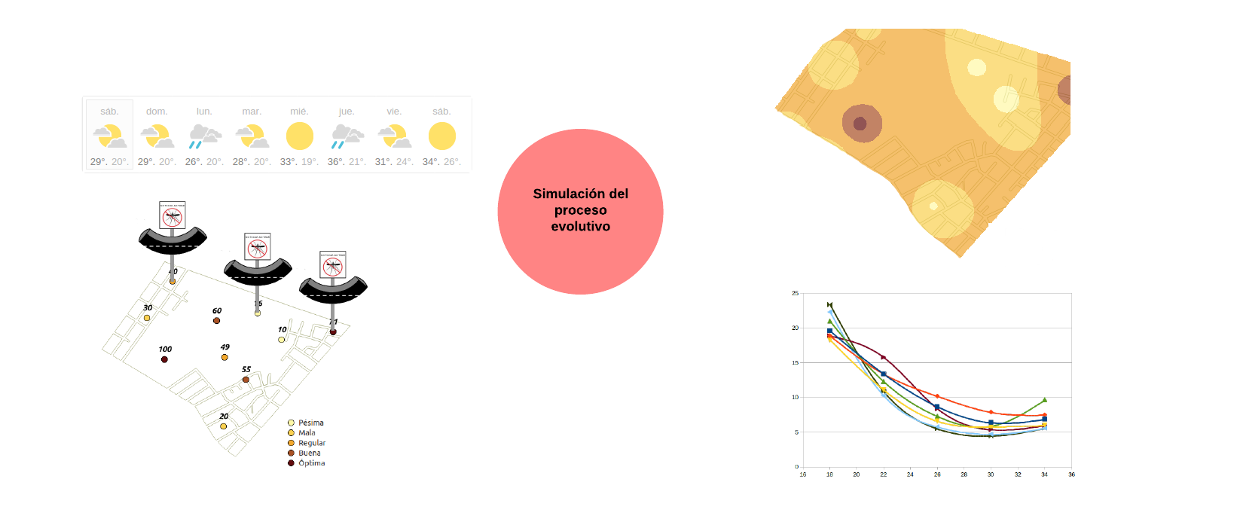
\includegraphics[width=\textwidth]{./graphics/propuesta.png}
  \end{center}
\end{frame}

\begin{frame}[c]{Preparación de datos de entrada}
  \begin{center}
    \begin{itemize}
      \item Selección del área de estudio.
      \item Distribución geográfica de los puntos de control.
      \item Revisión de los puntos de control.
      \item Generación de la población inicial a partir de los puntos de control.
      \item Obtener datos climáticos para el periodo de simulación.
      \item Conteo de larvas mediante Proceso Digital de imágenes.
    \end{itemize}
  \end{center}
\end{frame}

\begin{frame}[c]{Simulación del proceso evolutivo}
  \begin{center}
    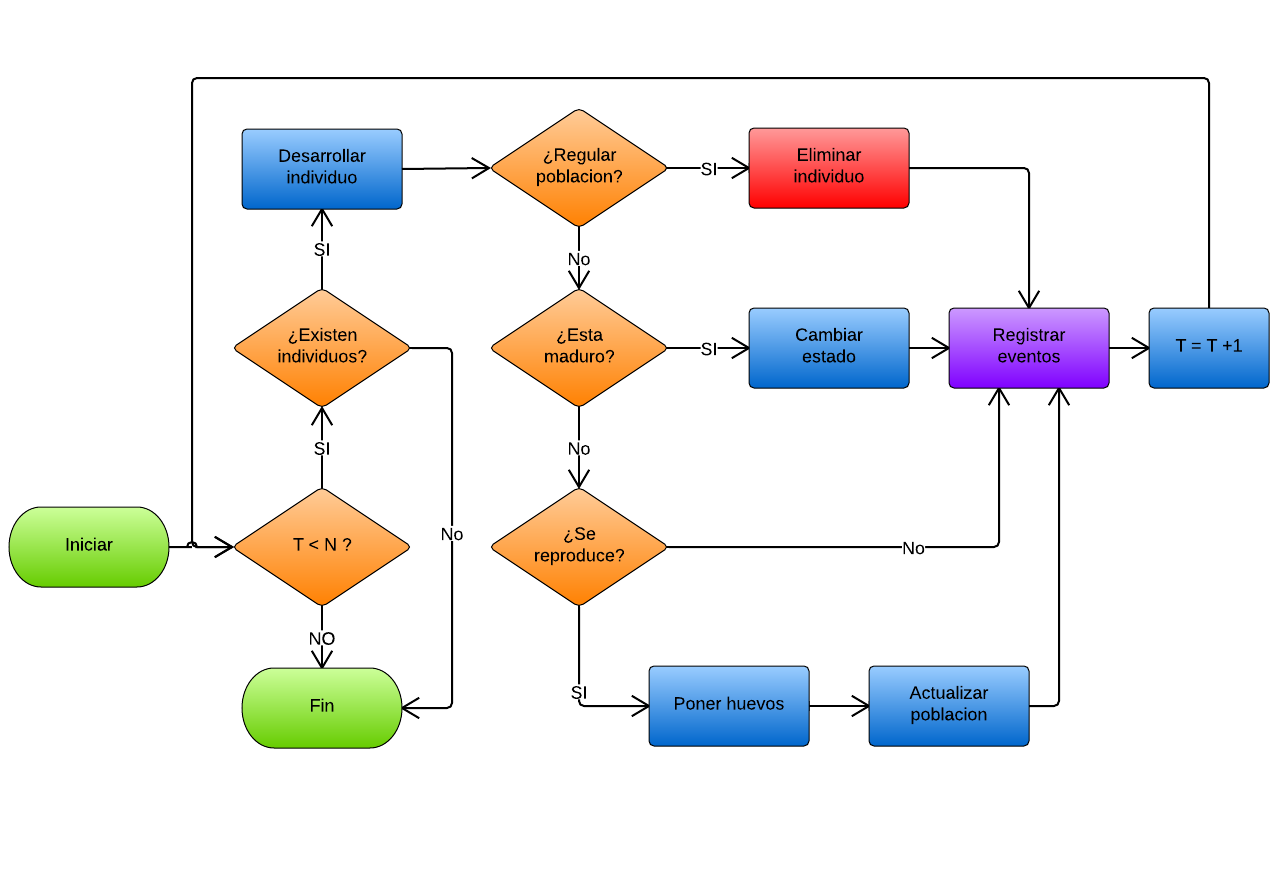
\includegraphics[height=7.5cm]{./graphics/algoritmo-propuesto.png}
  \end{center}
\end{frame}

\begin{frame}[c]{Simulación del proceso evolutivo. Ciclo de vida del vector.}
    \begin{columns}[t]
        \begin{column}[T]{7cm}
            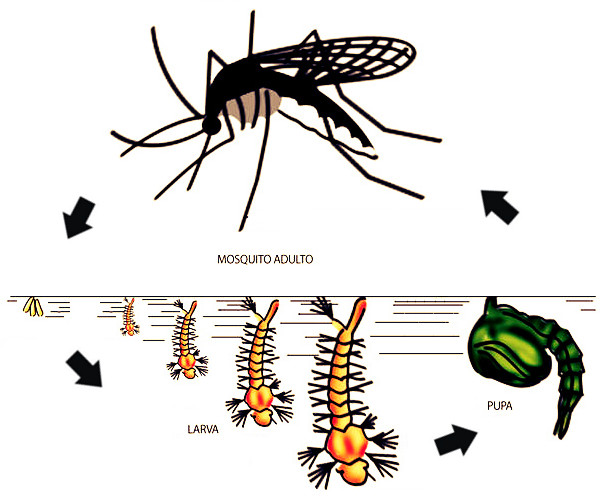
\includegraphics[width=7.5cm]{./graphics/ciclo-de-vida.jpg}
        \end{column}
        \begin{column}[T]{3cm}
          \begin{itemize}
            \item Desarrollo.
            \item Mortalidad.
            \item Dispersión.
            \item Ovipostura.
          \end{itemize}
        \end{column}
    \end{columns}
\end{frame}

\begin{frame}[c]{Simulación del proceso evolutivo. Tasas de desarrollo}
  \begin{itemize}

    \item Las tasas dependen no sólo de valores de la población, sino también de la temperatura lo que introduce una dependencia del tiempo.

    \item El cálculo de las tasas de desarrollo se realiza mediante el modelo no lineal de Sharpe y DeMichele.

    \item El modelo de Sharpe y DeMichele debe ajustarse con los datos biológicos disponibles.
    \item Una vez configurado, puede utilizarse para calcular tasas de desarrollo a cualquier temperatura.
  \end{itemize}
\end{frame}

\begin{frame}[c]{Simulación del proceso evolutivo. Tasas de desarrollo}
  \begin{center}
      \begin{equation} \label{eq:schoolfield}
         R(k)  = R(298K) *\cfrac{ \cfrac{k}{298K} *
          exp \Bigg[
                  \cfrac{\Delta H_{A}}{R} \bigg(\cfrac{1}{298K} - \cfrac{1}{k}\bigg)
              \Bigg]}
          {1 + exp\Bigg[\cfrac{\Delta H_{H}}{R} \bigg(\cfrac{1}{T_{1/2}}- \cfrac{1}{k}\bigg)\Bigg] }
      \end{equation}
  \end{center}
  Donde :
   \begin{itemize}
      \item $R(k)$ : Tasa de desarrollo media ($dias^{-1}$).
      \item $\Delta H_{A}$ y $\Delta H_{H}$ : son entalpías termodinámicas características del organismo.
      \item $T_{1/2}$ es la temperatura cuando la mitad de la enzima se desactiva.
      \item $R$ : es la constante universal de los gases.
      \item $k$ : Temperatura en Kelvin.
      \end{itemize}
\end{frame}

\begin{frame}[c]{Simulación del proceso evolutivo. Tasas de Mortalidad}
  \begin{itemize}
    \item Huevos, es definida como una constante.
    \item Larvas, expresada como una función, influenciada por la mortalidad bajo óptimas condiciones y la mortalidad denso dependiente.
    \item Pupas, expresada como una función influenciada por la mortalidad bajo óptimas condiciones.
    \item Adultos, es definida como una constante.
  \end{itemize}
\end{frame}

\begin{frame}[c]{Simulación del proceso evolutivo. Mortalidad}
  Mortalidad de los huevos :
  \begin{center}
      \begin{equation}
          M_{H(x,y)} = me * H(x,y)
      \end{equation}
  \end{center}
  Donde :
    \begin{itemize}
      \item $me$ : Tasa de mortalidad diaria igual a $0,01$ \ $1/\text{días}$.
      \item $H(x, y)$ : Cantidad de huevos observados en $(x,y)$.
      \item $M_{H(x,y)}$ : Cantidad de huevos a eliminar.
    \end{itemize}
\end{frame}

\begin{frame}[c]{Simulación del proceso evolutivo. Mortalidad.}
  Mortalidad bajo optimas condiciones de las larvas y pupas :
  \begin{center}
    \begin{equation}
    \label{eq:mortalidad-natural-larvas}
        mo(k) = 0.01 + 0.9725 * exp\bigg( \frac{-(k - 278)}{2.7035}\bigg)
    \end{equation}
  \end{center}
  Donde :
    \begin{itemize}
      \item $k$ : Temperatura en Kelvin.
    \end{itemize}
\end{frame}

\begin{frame}[c]{Simulación del proceso evolutivo. Mortalidad.}
  Mortalidad de las larvas :
  \begin{center}
      \begin{equation}
      M_{L(x,y)}(k) = mo(k) * L(x,y) + \bigg(\frac{\alpha _{0}}{BS(x,y)}\bigg) * L(x,y) *(L(x,y) - 1)
    \end{equation}
  \end{center}
  Donde:
 \begin{itemize}
      \item $k$ : Temperatura en Kelvin.
      \item $L(x, y)$ : Cantidad de larvas observadas en $(x,y)$.
      \item $\alpha _{0}$ : Capacidad de carga de un solo lugar de reproducción.
      \item $BS(x,y)$ : Es el número de sitios de reproducción en $(x,y)$ .
      \item $M_{L(x,y)}$ : Cantidad de larvas a eliminar.
    \end{itemize}
\end{frame}

\begin{frame}[c]{Simulación del proceso evolutivo. Mortalidad.}
  Mortalidad de las pupas :
  \begin{center}
    \begin{equation}
        M_{P(x,y)}(k) = P(x,y) * (mo(k) + (1 - ef) * R(k))
    \end{equation}
  \end{center}
  Donde :
    \begin{itemize}
      \item $k$ : Temperatura en Kelvin.
      \item $ef$ : el factor de supervivencia es de $0,83$.
      \item $P(x, y)$ : Cantidad de pupas observadas en $(x,y)$.
      \item $M_{P(x,y)}$ : Cantidad de pupas a eliminar.
    \end{itemize}
\end{frame}

\begin{frame}[c]{Simulación del proceso evolutivo. Mortalidad.}
  Mortalidad de adultos :
  \begin{center}
    \begin{equation}
        M_{A(x,y)} = ma * A(x,y)
    \end{equation}
  \end{center}
  Donde:
    \begin{itemize}
      \item $ma$ : Tasa de mortalidad diaria igual a $0,09$ \ $1/\text{días}$.
      \item $A(x, y)$ : Cantidad de adultos observados en $(x,y)$.
      \item $M_{A(x,y)}$ : Cantidad de adultos a eliminar.
    \end{itemize}
\end{frame}

\begin{frame}[c]{Simulación del proceso evolutivo. Ciclo gonotrófico y Ovipostura.}
  \begin{center}
      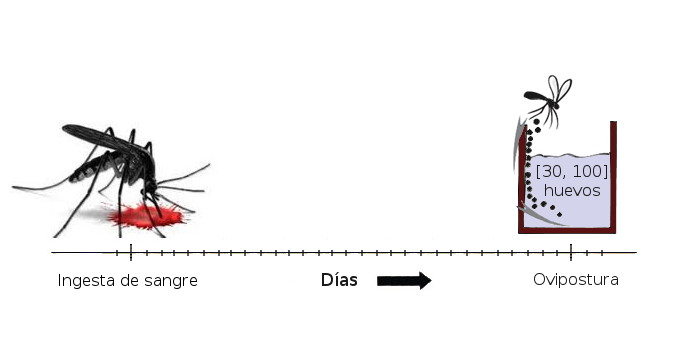
\includegraphics[width=\textwidth]{./graphics/cliclo-gonotrofico-tiempo.jpg}
  \end{center}
\end{frame}

\begin{frame}[c]{Simulación del proceso evolutivo. Dispersión.}
  \begin{center}
    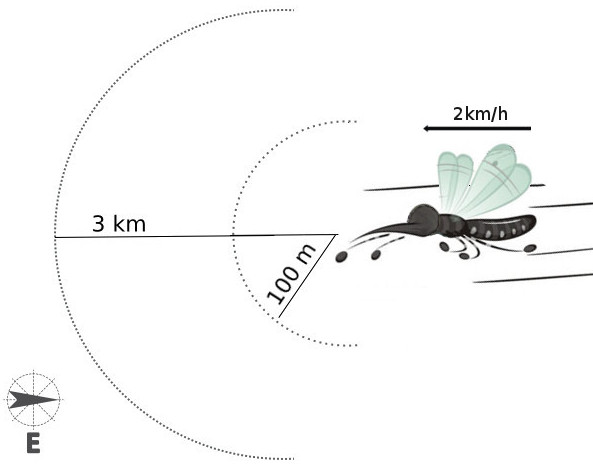
\includegraphics[width=8.5cm]{./graphics/dispersion.jpg}
  \end{center}
\end{frame}

\begin{frame}[c]{Clasificación de los niveles de infestación.}
  \begin{table}
    \begin{minipage}{\textwidth}
    \begin{center}
    \caption{\label{tab:cap4-puntaje-zona} Escala de clasificación de los niveles de infestación teniendo en cuenta la cantidad de larvas.}
      \begin{tabular}{l c c c c}
          \hline
                       &          &           & Hembras     & Hembras \\
          Tipo de zona &Mínimo$^a$& Máximo$^a$& Adultas$^b$ & Reproductivas $^c$\\
          \hline
          \hline
          Muy baja  & 0  & 19 & 8  & 5 \\
          Baja    & 20 & 35 & 15 & 10\\
          Normal & 36 & 51 & 22 & 15\\
          Alta   & 52 & 69 & 30 & 20\\
          Muy alta  & 70 & --$^d$  & --$^d$  & --$^d$ \\
      \end{tabular}
      \footnotetext[1]{Rango mínimo y máximo permitido el nivel.}
      \footnotetext[2]{Cantidad máxima de hembras adultas, al final del periodo de desarrollo.}
      \footnotetext[3]{Cantidad de hembras adultas con capacidad de oviponer.}
      \footnotetext[4]{No se estableció un límite superior para las niveles muy altos. }
      \end{center}
    \end{minipage}
  \end{table}
\end{frame}

\begin{frame}[t]{Clasificación de los niveles de infestación.}
  Consideraciones para la clasificación de los niveles de infestación:
  \begin{itemize}
      \item Solo el $50$ \% de las larvas observadas son hembras.
      \item La temperatura media anual es de 25 \textcelsius.
      \item La tasa mortalidad diaria natural de las larvas y pupas bajo optimas condiciones, a 25 \textcelsius, es igual a $0,01056$ 1/días respectivamente.
      \item La tasa de desarrollo, a 25 \textcelsius, de la larva hasta su emergencia a adulto es de $11,57$ días.
      \item El $32,10$ \% de las hembras adultas no oviponen.
  \end{itemize}
\end{frame}

\begin{frame}[c]{Análisis y presentación de los resultados}
  \begin{center}
      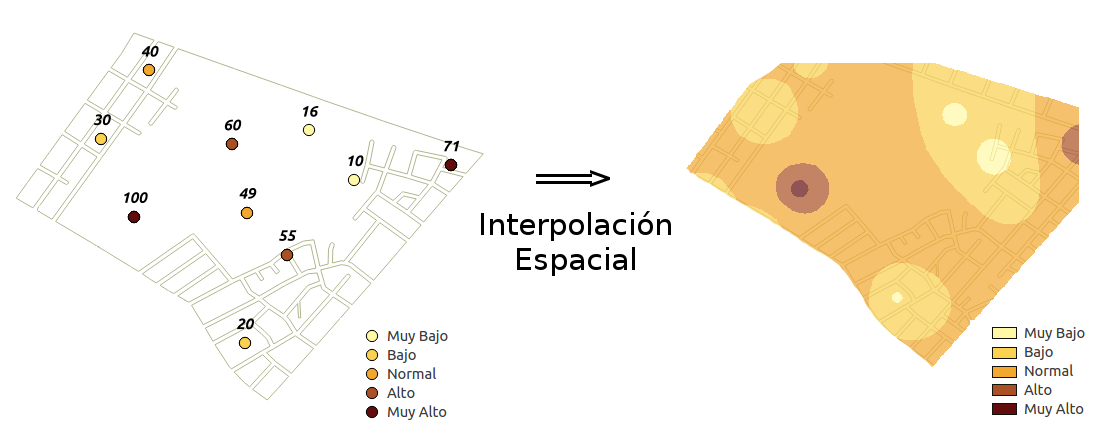
\includegraphics[width=\textwidth]{./graphics/identificacion-focos.png}
  \end{center}
\end{frame}

\begin{frame}[t]{Análisis y presentación de los resultados}
  \begin{center}
      \begin{itemize}
        \item Tasa promedio de desarrollo.
        \item Tasa promedio de mortalidad diaria.
        \item Cantidad promedio de huevos.
        \item Dispersión media.
        \item Cartografía del vector.
        \item Mapas de interpolación.
      \end{itemize}
  \end{center}
\end{frame}
